% =============================================================================
% ch06_algorithm.tex — Chapter 6: Proposed Algorithm | Biomimetic Navigator
% =============================================================================

\selectlanguage{hebrew}
\section{האלגוריתם הביומימטי המוצע}
\label{sec:algorithm}

\subsection{סקירה כללית של צינור ה-\en{BioSLAM}}
האלגוריתם המרכזי בעבודה זו, המכונה \en{BioSLAM}, שואף לחקות את תהליך העיבוד המוחי של העטלף ולהטמיע אותו בתוך מסגרת \en{SLAM} מודרנית. המערכת פועלת במעגל סגור של פליטת אות, קליטה, עיבוד ועדכון מפה.

\subsection{שלב הפליטה: יצירת פולס \en{LFM} סינתטי}
המערכת מייצרת פולס \en{LFM} (\en{Linear Frequency Modulated}) בתדרים אולטרה-סוניים. פונקציית הגל $s(t)$ מוגדרת כ:
\begin{equation}
    s(t) = \sin\left(2\pi \left(f_0 t + \frac{B}{2T}t^2\right)\right), \quad 0 \le t \le T
    \label{eq:lfm_gen}
\end{equation}
כאשר $f_0$ הוא תדר ההתחלה, $B$ רוחב הפס ו-$T$ משך פולס.

\subsection{שלב הקבלה: עיבוד באמצעות מסנן-מתואם (\en{Matched Filter})}
כדי לחלץ את המרחק למכשול בדיוק מקסימלי, אנו מבצעים קורלציה צולבת בין האות המוחזר לאות המשודר. רזולוציית הטווח $\Delta r$ תלויה ישירות ברוחב הפס $B$:
\begin{equation}
    \Delta r = \frac{c}{2B}
    \label{eq:range_res}
\end{equation}
עבור רוחב פס של 80 \en{kHz}, אנו מקבלים רזולוציה של כ-2.1 מ"מ, המאפשרת זיהוי מכשולים עדינים כגון ענפים או כבלים. \cite{Rihaczek1969MatchedFilter}

\subsection{השוואה ביומימטית: עטלף מול רחפן}
איור \ref{fig:bat_vs_artificial} מציג את ההקבלה בין שלבי העיבוד הביולוגי לבין המימוש המלאכותי שלנו:

\begin{figure}[H]
    \centering
    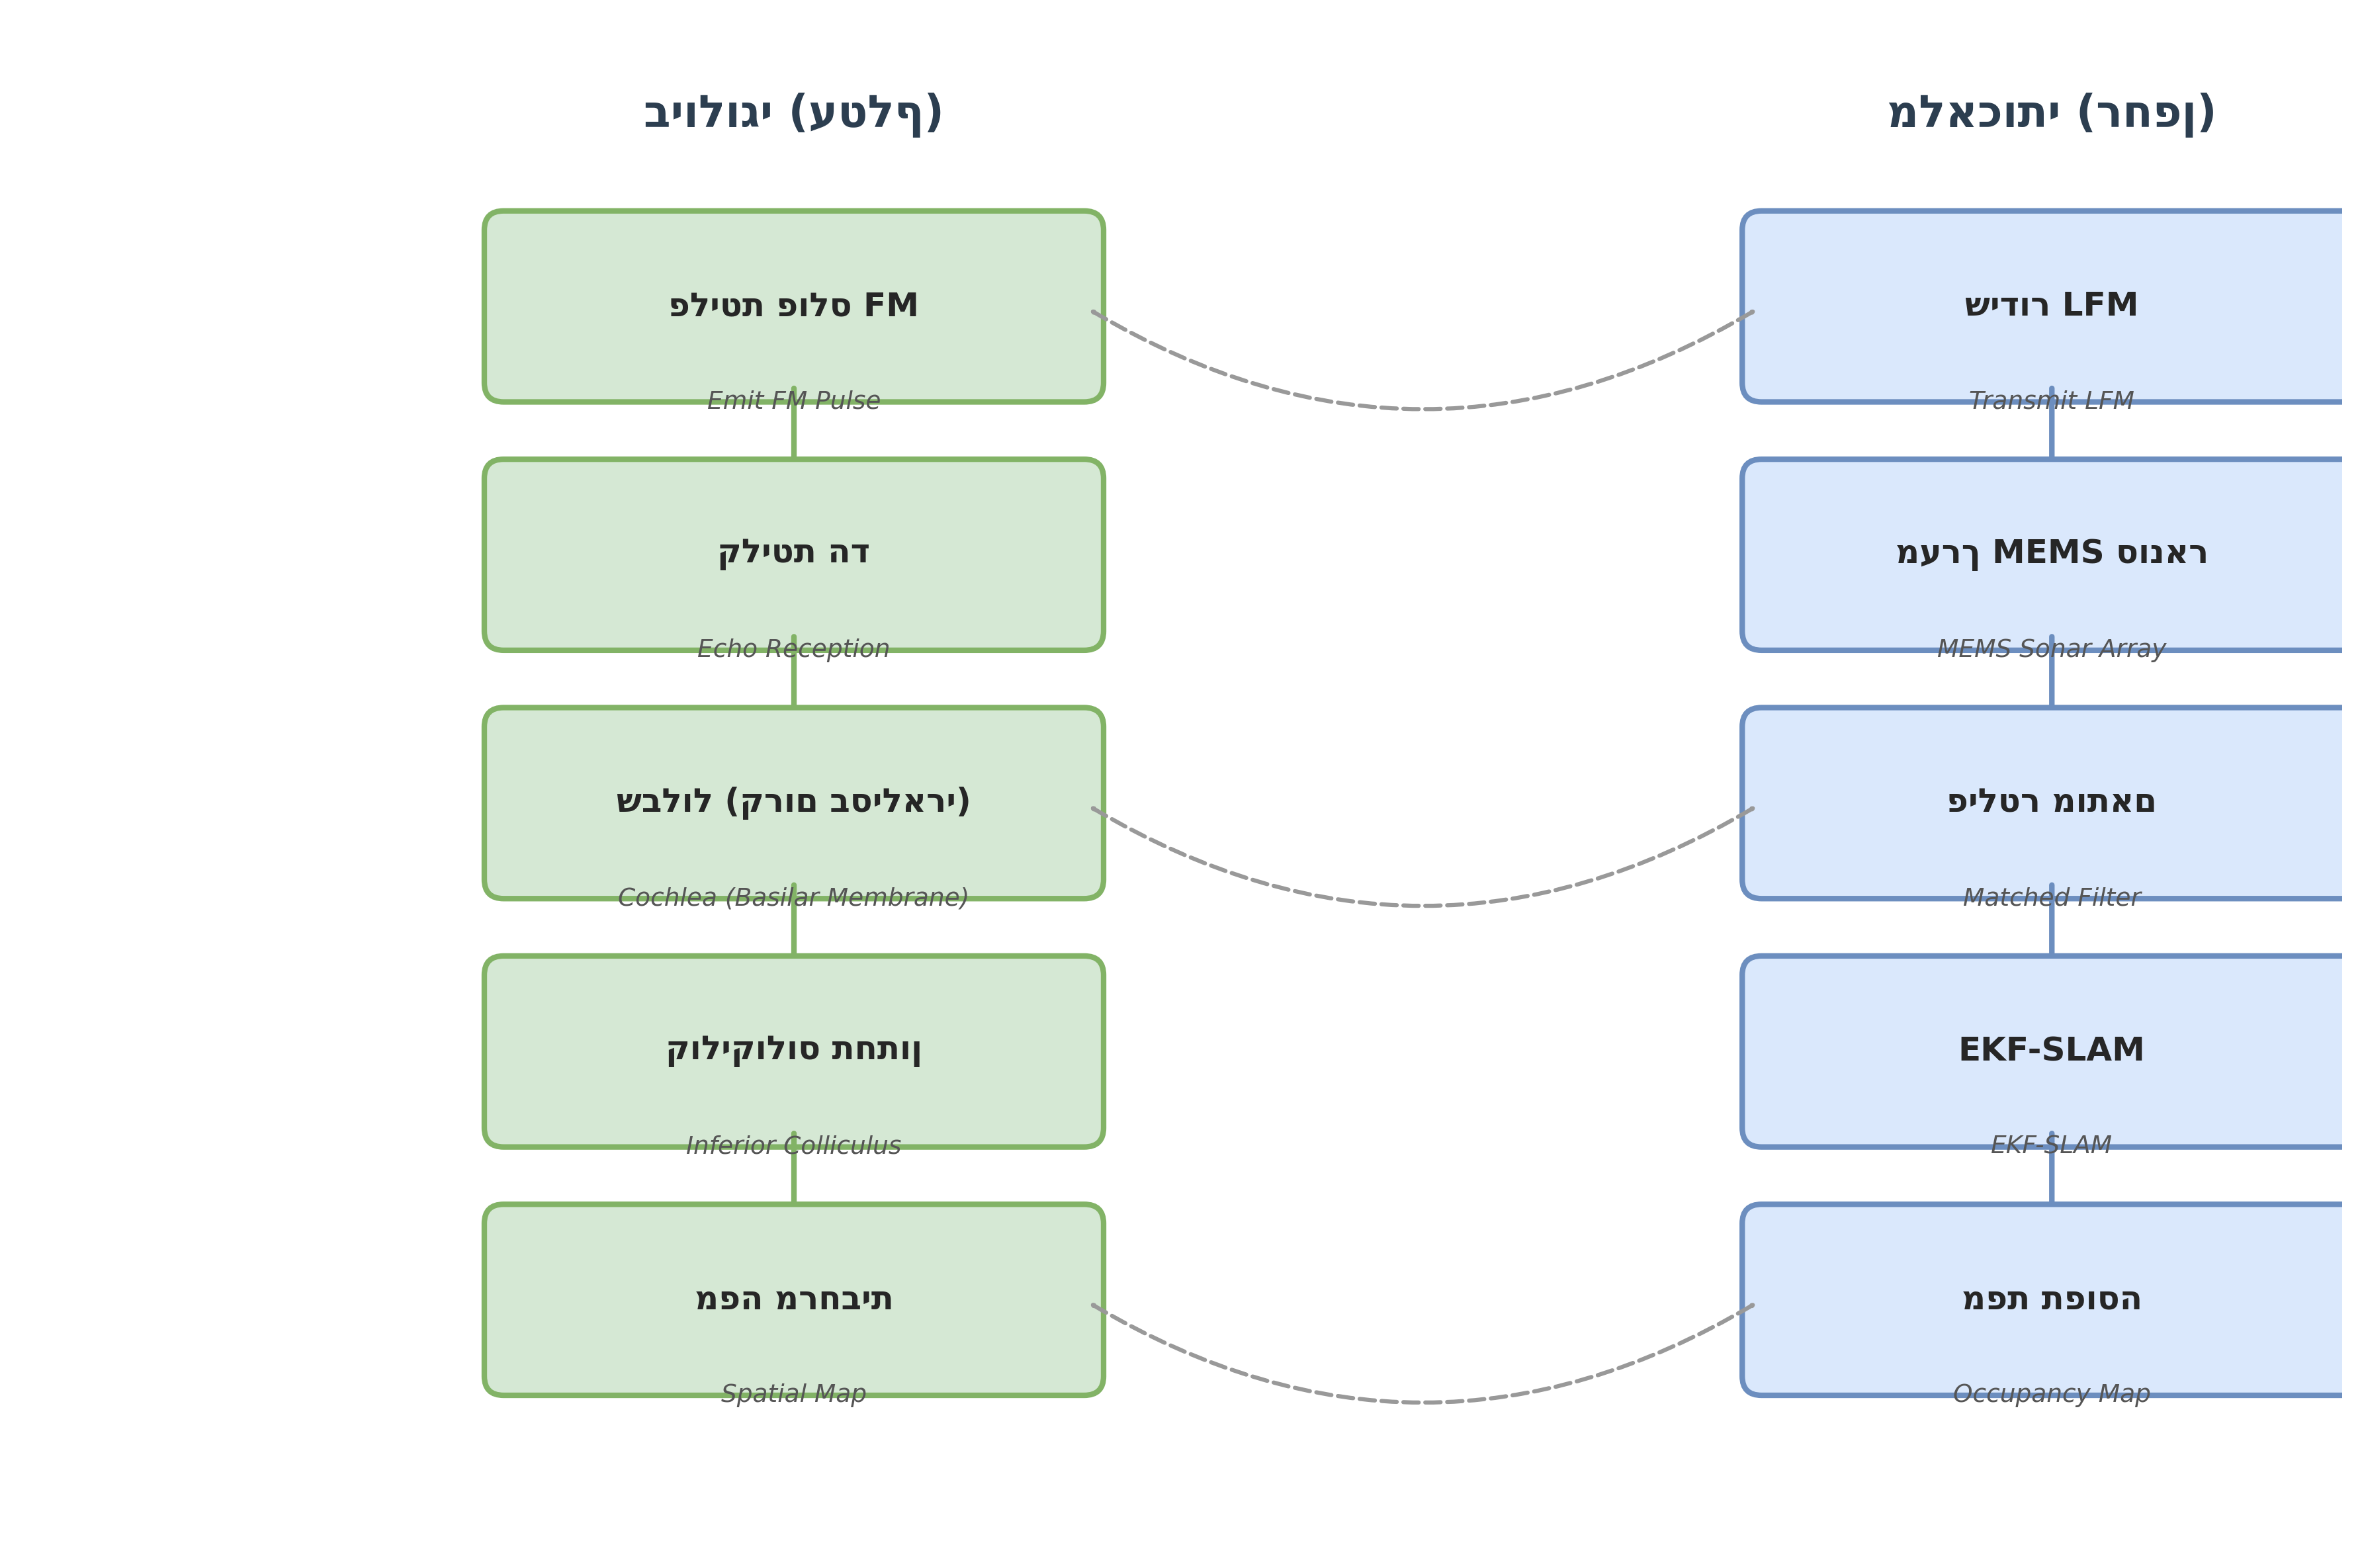
\includegraphics[width=0.9\columnwidth]{figures/fig_bat_vs_artificial.png}
    \caption{השוואת מסלולי העיבוד: אקולוקציה ביולוגית (למעלה) לעומת הצינור המלאכותי של \en{BioSLAM} (למטה).}
    \label{fig:bat_vs_artificial}
\end{figure}

\subsection{אינטגרציה עם מסנן קלמן מורחב}
המדידות המופקות מהסונאר משולבות בתוך \en{EKF} כחלק מוקטור התצפיות. פונקציית התצפית $h(\mathbf{x})$ עבור חיישן הממוקם ב-$(x_s, y_s)$ המזהה מכשול ב-$(x_m, y_m)$ היא:
\begin{equation}
    h(\mathbf{x}) = \sqrt{(x_m - x_s)^2 + (y_m - y_s)^2}
    \label{eq:obs_model}
\end{equation}
היעקוביאנים של פונקציה זו מחושבים בזמן אמת כדי לעדכן את מטריצת הקווריאנס של הרחפן.
